% define documentclass
\documentclass[12pt, bibliography=totoc, a4paper, abstractoff, numbers=noenddot]{scrreprt}

% define used packages
\usepackage[left=4.0cm, right=2.0cm, top=3cm, bottom=3cm]{geometry}
\usepackage{bibgerm}
\usepackage[utf8]{inputenc}
\usepackage[T1]{fontenc}
\usepackage{graphicx}
\usepackage[ngerman]{babel}
\usepackage{lmodern}
\usepackage{listings}
\usepackage[numbers]{natbib}
\usepackage{acronym}
\bibliographystyle{alphadin}
\usepackage{float}

\usepackage{lastpage}

% advanced tables
\usepackage{array}

% header and footer
\usepackage{fancyhdr}

% links
\usepackage{url}

% internal links
\usepackage[colorlinks=true ,linkcolor=black,
			anchorcolor=black ,citecolor=black ,filecolor=black,
			menucolor=black ,urlcolor=black]{hyperref}

% mathematical formulas
\usepackage{amsmath, amssymb}

% fancy Diagrams %
\usepackage{tikz}
\usepackage{epstopdf}

% to include images side by side
\usepackage{subfigure}

% for nice bg on title page
\usepackage{eso-pic}
\newcommand\BackgroundPic{%
\put(0,0){%
\parbox[b][\paperheight]{\paperwidth}{%
\vfill
\centering

\includegraphics[width=\paperwidth,height=\paperheight,%
keepaspectratio]{images/Logo_H-BRS_background}%
\vfill
}}}

% define the programming language
\usepackage{listings}
\lstloadlanguages{Java,sh,bash,Haskell,HTML,PHP,XML}
\lstdefinelanguage{console}{
  morekeywords={},
  otherkeywords={warumgehtdasnicht>,\$}
}
\newcommand{\lstsetconsole}
{ \lstset{%language=sh,
        lineskip=-2pt,
        breaklines=true,
        language=console,
        breaklines=true,
        captionpos=b,
        commentstyle=\textit,
        keywordstyle=\bfseries,
        basicstyle=\ttfamily,
        stringstyle=\ttfamily,
        showstringspaces=false,
        frame=single,
        tabsize=2
  }
}
\lstdefinelanguage{scalaconsole}{
  morekeywords={},
  otherkeywords={scala>,\|}
}
\newcommand{\lstsetrepl}
{ \lstset{%language=sh,
        lineskip=-2pt,
        breaklines=true,
        language=scalaconsole,
        breaklines=true,
        commentstyle=\textit,
        keywordstyle=\bfseries,
        basicstyle=\ttfamily,
        stringstyle=\ttfamily,
        showstringspaces=false,
        frame=single,
        tabsize=2
  }
}
\newcommand{\lstsetjava}{
 \lstset{language=Java,
        breaklines=true,
        commentstyle=\textit,
        keywordstyle=\bfseries,
        basicstyle=\ttfamily,
        stringstyle=\ttfamily,
        showstringspaces=false,
        frame=single,
        captionpos=b,
        tabsize=2,
        literate=
        %linewidth=\textwidth,captionpos=b
        %numbers=left, stepnumber=5, numbersep=10pt
 }
}
\lstdefinelanguage{scala}{
  morekeywords={abstract,case,catch,class,def,%
    do,else,extends,false,final,finally,%
    for,forSome,if,implicit,import,lazy,match,mixin,%
    new,null,object,override,package,%
    private,protected,requires,return,sealed,%
    super,this,throw,trait,true,try,%
    type,val,var,while,with,yield},
  otherkeywords={_,:,=,=>,<-,<\%,<:,>:,\#,@},
  sensitive=true,
  morecomment=[l]{//},
  morecomment=[n]{/*}{*/},
  morestring=[b]",
  morestring=[b]',
  morestring=[b]"""
}
\newcommand{\lstsetscala}{
 \lstset{language=scala,
        breaklines=true,
        commentstyle=\textit,
        keywordstyle=\bfseries,
        basicstyle=\ttfamily,
        stringstyle=\ttfamily,
        showstringspaces=false,
        frame=single,
        tabsize=2
        %%linewidth=\textwidth,captionpos=b
        %numbers=left, stepnumber=5, numbersep=10pt
 }
}
\newcommand{\lstsethtml}{
 \lstset{language=HTML,
        breaklines=true,
        commentstyle=\textit,
        keywordstyle=\bfseries,
        basicstyle=\ttfamily,
        stringstyle=\ttfamily,
        showstringspaces=false,
        frame=single,
        tabsize=2
        %%linewidth=\textwidth,captionpos=b
        %numbers=left, stepnumber=5, numbersep=10pt
 }
}
\newcommand{\lstsetphp}{
 \lstset{language=PHP,
        breaklines=true,
        commentstyle=\textit,
        keywordstyle=\bfseries,
        basicstyle=\ttfamily,
        stringstyle=\ttfamily,
        showstringspaces=false,
        frame=single,
        tabsize=2
        %%linewidth=\textwidth,captionpos=b
        %numbers=left, stepnumber=5, numbersep=10pt
 }
}
\lstnewenvironment{code}
    {\lstset{}%
      \csname lst@SetFirstLabel\endcsname}
    {\csname lst@SaveFirstLabel\endcsname}
\newcommand{\lstsethaskell}{
    \lstset{
      language=Haskell,
      commentstyle=\textit,
      keywordstyle=\bfseries,
      basicstyle=\ttfamily,
      stringstyle=\ttfamily,
      showstringspaces=false,
      frame=single,
      flexiblecolumns=false,
      basewidth={0.5em,0.45em},
      literate={+}{{$+$}}1 {/}{{$/$}}1 {*}{{$*$}}1 {=}{{$=$}}1
               {==}{{$==$}}2 %{!=}{{$\not\equiv$}}2
               {>}{{$>$}}1 {<}{{$<$}}1 {\\}{{$\lambda$}}1
               {\\\\}{{\char`\\\char`\\}}1
               {->}{{$\rightarrow$} }2 {>=}{{$\geq$}}2 {<-}{{$\leftarrow$}}2
               {<=}{{$\leq$}}2 {=>}{{$\Rightarrow$} }2
               {\ .}{{$\circ$}}2 {\ .\ }{{$\circ$}}2 {(.)}{({$\circ$})}2
               {>>}{{>>}}2 {>>=}{{>>=}}2
               {|}{{$\mid$}}1
    }
}
\lstdefinelanguage{JavaScript}{
  keywords={typeof, new, true, false, catch,%
    function, return, null, catch, switch, var,%
    if, in, while, do, else, case, break},
  ndkeywords={class, export, boolean, throw, implements, import, this},
  sensitive=false,
  comment=[l]{//},
  morecomment=[s]{/*}{*/},
  morestring=[b]',
  morestring=[b]"
}
\newcommand{\lstsetjavascript}{
  \lstset{
		language=JavaScript,
		breaklines=true,
		commentstyle=\textit,
		basicstyle=\ttfamily,
		keywordstyle=\bfseries,
		stringstyle=\ttfamily,
		showstringspaces=false,
		frame=single,
		tabsize=2
  }
}
\newcommand{\lstsetxml}{
 \lstset{language=XML,
        breaklines=true,
        commentstyle=\sffamily,
        keywordstyle=\bfseries,
        basicstyle=\sffamily,
        showstringspaces=false,
        stringstyle=\ttfamily,
        frame=single,
        tabsize=2,
        literate=
        %linewidth=\textwidth,captionpos=b
        %numbers=left, stepnumber=5, numbersep=10pt
 }
}
\lstdefinelanguage{CSharp}{
 morekeywords = {abstract,event,new,struct,as,explicit,%
    null,switch,base,extern,object,this,bool,false,%
    operator,throw,break,finally,out,true,byte,fixed,%
    override,try,case,float,params,typeof,catch,for,%
    private,uint,char,foreach,protected,ulong,checked,%
    goto,public,unchecked,class,if,readonly,unsafe,%
    const,implicit,ref,ushort,continue,in,return,using,%
    decimal,int,sbyte,virtual,default,interface,sealed,%
    volatile,delegate,internal,short,void,do,is,sizeof,%
    while,double,lock,stackalloc,else,long,static,%
    enum,namespace,string,partial},
  morecomment = [l]{//},
  morecomment = [l]{///},
  morecomment = [s]{/*}{*/},
  morestring=[b]",
  sensitive = true
}
\newcommand{\lstsetcsharp}{
 \lstset{language=csharp,
        breaklines=true,
        commentstyle=\sffamily,
        basicstyle=\sffamily,
        keywordstyle=\bfseries,
        stringstyle=\ttfamily,
        showstringspaces=false,
        frame=single,
        tabsize=2
        %%linewidth=\textwidth,captionpos=b
        %numbers=left, stepnumber=5, numbersep=10pt
 }
}
\lstdefinelanguage{FSharp}{
  morekeywords={abstract,and,as,assert,base,begin,%
    class,default,delegate,do,done,downcast,downto,%
    elif,else,end,exception,extern,false,finally,for,fun,%
    function,if,in,inherit,inline,interface,internal,lazy,%
    let,match,member,module,mutable,namespace,%
    new,not,null,of,open,or,override,private,public,rec,%
    return,static,struct,then,to,true,try,type,upcast,use,%
    val,void,when,while,with,yield,asr,land,lor,lsl,lsr,lxor,%
    mod,sig,atomic,break,checked,component,const,%
    constraint,constructor,continue,eager,event,external,%
    fixed,functor,global,include,method,mixin,object,%
    parallel,process,protected,pure,sealed,tailcall,trait,virtual,volatile},     
  sensitive=false,
  morecomment=[l][\color{greencomments}]{///},
  morecomment=[l][\color{greencomments}]{//},
  morecomment=[s][\color{greencomments}]{{(*}{*)}},
  morestring=[b]"
}
\newcommand{\lstsetfsharp}{
 \lstset{language=fsharp,
        breaklines=true,
        commentstyle=\sffamily,
        basicstyle=\sffamily,
        keywordstyle=\bfseries,
        stringstyle=\ttfamily,
        showstringspaces=false,
        frame=single,
        tabsize=2
        %%linewidth=\textwidth,captionpos=b
        %numbers=left, stepnumber=5, numbersep=10pt
 }
}

%set default pagestyle
\pagestyle{empty}

\setlength{\parindent}{0pt}
\setlength{\parskip}{12pt}

% #####
% #
% # START config area
% #
% #####

\newcommand{\HEADER}[0]{H-BRS, WS 2016 / 2017}
\newcommand{\PAGENUMBERS}[0]{\pagemark}
\newcommand{\DATE}[0]{06.11.2016}

\newcommand{\AUTHOR}[0]{Franz-Dominik Dahmann}
\newcommand{\MATNR}[0]{9019745}
\newcommand{\STREET}[0]{Münchhausenweg 30}
\newcommand{\ZIP}[0]{53340}
\newcommand{\TOWN}[0]{Meckenheim}

\newcommand{\REFERENT}[0]{Prof. Dr. Knolle} 
\newcommand{\KOREFERENT}[0]{B. Mager}

\newcommand{\TITLE}[0]{MongoDB als Datenbank für Document Stores}
\newcommand{\COURSE}[0]{Studiengang MCS}
\newcommand{\TYPE}[0]{Schemalose Datenbank}
\newcommand{\COMPLETION}[0]{Master of Science}

% #####
% #
% # END config area
% #
% #####

% Hurenkinder und Schusterjungenregelung
\clubpenalty=100000
\widowpenalty=100000
\displaywidowpenalty=100000

% starting the document
\begin{document}

% set pagenumbering to roman(I II III IV)
\pagenumbering{Roman}
% input the title
% #####
% #
% # This is the titlelayout from Prof. Dr. Harm Knolle 
% # (Hochschule Bonn-Rhein-Sieg)
% #  
% #####

% #####
% #
% # Default layout
% #
% #####

\AddToShipoutPicture*{\BackgroundPic}

\begin{titlepage}
  \begin{center}
  	
\includegraphics[scale=1]{./images/Logo_H-BRS.jpg}
  \end{center}
  \vspace{40pt}
  \sffamily
  \begin{tabular}{|l>{\raggedright\hspace{0pt}\arraybackslash}p{15cm}}
    & \\
    & \large\textbf{\TYPE}\\[\baselineskip]
    & \huge\textbf{\TITLE}\\[\baselineskip]
    & \textbf{Falls erforderlich: Zur Erlangung des akademischen Grades eines}\\ 
    & \COMPLETION\\
    & - \COURSE\ -\\
    & \\
  \end{tabular}
  \vfill
  \begin{tabular}{ll@{}}
    & Fachbereich Informatik\\[\baselineskip]
    &   Referent: \REFERENT\\[\baselineskip]
    &   Falls erforderlich: Korreferent: \KOREFERENT\\[\baselineskip]
    & \\[\baselineskip]
    & eingereicht von:\\[\baselineskip]
    & \AUTHOR\\[\baselineskip]
    & Matr.-Nr. \MATNR\\[\baselineskip]
    & \STREET\\[\baselineskip]
    & \ZIP \ \TOWN\\[\baselineskip]
    & \\[\baselineskip]
    & Sankt Augustin, den \DATE\\[\baselineskip]
  \end{tabular}
\end{titlepage}


\begin{abstract}
\section*{Zusammenfassung}\markboth{Zusammenfassung}{}
  \addcontentsline{toc}{chapter}{Zusammenfassung}Lorem ipsum dolor sit amet, consetetur sadipscing elitr, sed diam nonumy eirmod tempor invidunt ut labore et dolore magna aliquyam erat, sed diam voluptua. At vero eos et accusam et justo duo dolores et ea rebum. Stet clita kasd gubergren, no sea takimata sanctus est Lorem ipsum dolor sit amet. Lorem ipsum dolor sit amet, consetetur sadipscing elitr, sed diam nonumy eirmod tempor invidunt ut labore et dolore magna aliquyam erat, sed diam voluptua. At vero eos et accusam et justo duo dolores et ea rebum. Stet clita kasd gubergren, no sea takimata sanctus est Lorem ipsum dolor sit amet. Lorem ipsum dolor sit amet, consetetur sadipscing elitr, sed diam nonumy eirmod tempor invidunt ut labore et dolore magna aliquyam erat, sed diam voluptua. At vero eos et accusam et justo duo dolores et ea rebum. Stet clita kasd gubergren, no sea takimata sanctus est Lorem ipsum dolor sit amet. 

Duis autem vel eum iriure dolor in hendrerit in vulputate velit esse molestie consequat, vel illum dolore eu feugiat nulla facilisis at vero eros et accumsan et iusto odio dignissim qui blandit praesent luptatum zzril delenit augue duis dolore te feugait nulla facilisi. Lorem ipsum dolor sit amet, consectetuer adipiscing elit, sed diam nonummy nibh euismod tincidunt ut laoreet dolore magna aliquam erat volutpat. 

Ut wisi enim ad minim veniam, quis nostrud exerci tation ullamcorper suscipit lobortis nisl ut aliquip ex ea commodo consequat. Duis autem vel eum iriure dolor in hendrerit in vulputate velit esse molestie consequat, vel illum dolore eu feugiat nulla facilisis at vero eros et accumsan et iusto odio dignissim qui blandit praesent luptatum zzril delenit augue duis dolore te feugait nulla facilisi. 

Nam liber tempor cum soluta nobis eleifend option congue nihil imperdiet doming id quod mazim placerat facer possim assum. Lorem ipsum dolor sit amet, consectetuer adipiscing elit, sed diam nonummy nibh euismod tincidunt ut laoreet dolore magna aliquam erat volutpat. Ut wisi enim ad minim veniam, quis nostrud exerci tation ullamcorper suscipit lobortis nisl ut aliquip ex ea commodo consequat. 

Duis autem vel eum iriure dolor in hendrerit in vulputate velit esse molestie consequat, vel illum dolore eu feugiat nulla facilisis. 
\end{abstract}

\cite{edlich01}
\cite{sadalage01}
\cite{redmont01}
\cite{Jing01}
\cite{Bogdan01}
\cite{Meier01}
\cite{Fasel01}
\cite{Meier02}
\cite{Fasel02}
\cite{Boicea01}
\cite{Parker01}
\cite{Abramova01}
\cite{Faraj01}
\cite{Shakuntala01}
\cite{Hows01}
\cite{fowler01}

% load the preamble
%% \renewcommand\abstractname{Danksagung}
\begin{abstract}
\section*{Vorwort}\markboth{Vorwort}{}
  \addcontentsline{toc}{chapter}{Vorwort}Lorem ipsum dolor sit amet, consetetur sadipscing elitr, sed diam nonumy eirmod tempor invidunt ut labore et dolore magna aliquyam erat, sed diam voluptua. At vero eos et accusam et justo duo dolores et ea rebum. Stet clita kasd gubergren, no sea takimata sanctus est Lorem ipsum dolor sit amet. Lorem ipsum dolor sit amet, consetetur sadipscing elitr, sed diam nonumy eirmod tempor invidunt ut labore et dolore magna aliquyam erat, sed diam voluptua. At vero eos et accusam et justo duo dolores et ea rebum. Stet clita kasd gubergren, no sea takimata sanctus est Lorem ipsum dolor sit amet. Lorem ipsum dolor sit amet, consetetur sadipscing elitr, sed diam nonumy eirmod tempor invidunt ut labore et dolore magna aliquyam erat, sed diam voluptua. At vero eos et accusam et justo duo dolores et ea rebum. Stet clita kasd gubergren, no sea takimata sanctus est Lorem ipsum dolor sit amet. 

Duis autem vel eum iriure dolor in hendrerit in vulputate velit esse molestie consequat, vel illum dolore eu feugiat nulla facilisis at vero eros et accumsan et iusto odio dignissim qui blandit praesent luptatum zzril delenit augue duis dolore te feugait nulla facilisi. Lorem ipsum dolor sit amet, consectetuer adipiscing elit, sed diam nonummy nibh euismod tincidunt ut laoreet dolore magna aliquam erat volutpat. 

Ut wisi enim ad minim veniam, quis nostrud exerci tation ullamcorper suscipit lobortis nisl ut aliquip ex ea commodo consequat. Duis autem vel eum iriure dolor in hendrerit in vulputate velit esse molestie consequat, vel illum dolore eu feugiat nulla facilisis at vero eros et accumsan et iusto odio dignissim qui blandit praesent luptatum zzril delenit augue duis dolore te feugait nulla facilisi. 

Nam liber tempor cum soluta nobis eleifend option congue nihil imperdiet doming id quod mazim placerat facer possim assum. Lorem ipsum dolor sit amet, consectetuer adipiscing elit, sed diam nonummy nibh euismod tincidunt ut laoreet dolore magna aliquam erat volutpat. Ut wisi enim ad minim veniam, quis nostrud exerci tation ullamcorper suscipit lobortis nisl ut aliquip ex ea commodo consequat. 

Duis autem vel eum iriure dolor in hendrerit in vulputate velit esse molestie consequat, vel illum dolore eu feugiat nulla facilisis. 
\end{abstract}


% loads the fancy pagestyle for register part
% set the pagestyle to fancy
\pagestyle{fancy}

\fancyhf{}% clear all fields
  % define the header
  \fancyhead[L]{\leftmark}% left header
  \fancyhead[R]{\HEADER}% right header
  \renewcommand{\headrulewidth}{0.4pt}% top line

  % define the footer
  \fancyfoot[L]{\AUTHOR}% left footer
  \fancyfoot[R]{\pagemark}% right footer
  \renewcommand{\footrulewidth}{0.6pt}% bottom line

  % redefine the chaptermark to have '1. Chaptername' and not 'CHAPTER 1.
  % CHAPTERNAME'
  \renewcommand{\chaptermark}[1]{\markboth{\thechapter.\ #1}{}}

% override the plain style
\fancypagestyle{plain}{%
\fancyhf{}% clear all fields
  % define the header
  \renewcommand{\headrulewidth}{0.0pt}% top line

  % define the footer
  \fancyfoot[L]{\AUTHOR}% left footer
  \fancyfoot[R]{\pagemark}% right footer
  \renewcommand{\footrulewidth}{0.6pt}% bottom line
}


% create the registers
\tableofcontents\newpage

% set pagenumbering to arabic(1 2 3 4)
\pagenumbering{arabic}
% loads the fancy pagestyle for main part
% set the pagestyle to fancy
\pagestyle{fancy}

\fancyhf{}% clear all fields
  % define the header
  \fancyhead[L]{\leftmark}% left header
  \fancyhead[R]{\HEADER}% right header
  \renewcommand{\headrulewidth}{0.4pt}% top line

  % define the footer
  \fancyfoot[L]{\AUTHOR}% left footer
  \fancyfoot[R]{\PAGENUMBERS}% right footer
  \renewcommand{\footrulewidth}{0.6pt}% bottom line

  % redefine the chaptermark to have '1. Chaptername' and not 'CHAPTER 1.
  % CHAPTERNAME'
  \renewcommand{\chaptermark}[1]{\markboth{\thechapter.\ #1}{}}

% override the plain style
\fancypagestyle{plain}{%
\fancyhf{}% clear all fields
  % define the header
  \renewcommand{\headrulewidth}{0pt}% top line

  % define the footer
  \fancyfoot[L]{\AUTHOR}% left footer
  \fancyfoot[R]{\PAGENUMBERS}% right footer
  \renewcommand{\footrulewidth}{0.6pt}% bottom line
}


% #####
% # load the chapter from the files
% #
% # TODO: create new chapter
% #####
\chapter{Ausgewählte Persistenzmodelle}
\section{Key-Value Stores}
\subsection{Einleitung}
Key-Value Stores oder Key-Value Datenbanken sind eine der einfachsten Formen der NoSQL Datenbanken. Sie können beliebige Werte (Englisch: Values) unter einem definierbaren Key persistieren und über diesen selektieren. Dabei können sie mit einem herkömmlichen relationalen Datenbanksystem (RDBS) verglichen werden in welchem die Tabellen nur zwei Attribute besitzen: eine ID- und eine Value-Spalte \cite{sadalage01}. Im Unterschied zu dieser relationalen Datenbank erwarten Key-Value Stores keinen Datentyp für den Value. Hier können beliebige Werte als blob gespeichert werden. Auch können Key-Value Datenbanken weder Relationen oder Beziehungen zwischen den Einträgen herstellen. Für die Semantik, Korrektheit der Werte, Beziehungen o.ä., ihre Verwendung, welcher Datentyp vorliegt und etwaiges Fehlerhandling ist allein die Anwendung, welche die Datenbank nutzt, verantwortlich. Dieses sehr grundlegende Verhalten soll eine möglichst hohe Performance und Skalierbarkeit ermöglichen. 

\subsection{Eigenschaften}
Einige Key-Value Stores gehen einen Schritt weiter und können das zu speichernde Aggregat differenzieren. So kann Redis beispielsweise Listen, Sets oder Hashes speichern und unterstützt einfache Operationen auf diesen Datenstrukturen. Somit verschwimmt in der Praxis der Unterschied zwischen Key-Value und Document Stores bei einigen Vertretern sehr.

Im Folgenden werden einige Eigenschaften von Key-Value Stores näher betrachtet und aufgezeigt wie diese sich von einem Standard RDBS unterscheiden.

\subsubsection{Konsistenz}
Da die Key-Value Datenbank Änderungen des Values nicht bestimmen kann, kann die Konsistenz somit nur über den Key und die damit verbundenen Operationen get, put oder delete gewährt werden \cite{sadalage01}. 

In verteilten System wird häufig die \textit{eventually consistent} Eigenschaft angewendet. 

\subsubsection{Transaktionen}
Für Transaktionen gibt es in der NoSQL Welt keine einheitliche Spezifikation. Jeder Anbieter von Key-Value Stores implementiert diese anders, Riak benutzt hier beispielsweise das Quorum-Konzept \cite{sadalage01}.

\subsubsection{Query-Eigenschaften}
Da sich Key-Value Datenbanken nicht für den gespeicherten Value interessieren kann man Queries nur auf den Key ausführen. Auf Grund dieses sehr einfachen Handlings sind Key-Value Stores nicht für Anwendungen geeignet, welche über den Inhalt filtern oder suchen müssen. Hier muss die Anwendung wissen welche Daten unter welchem Key zu finden sind und welchen Key sie aufrufen möchte. Da nicht immer der Fall eintritt, dass der Key zu einem Datum bekannt ist, stellen manche Key-Value Datenbanken allerdings eine Suchfunktionalität oder die Möglichkeit der Indexierung bereit, damit nicht jeder Datensatz von der Anwendung geladen und einzeln durchsucht werden muss \cite{sadalage01}. 

\subsubsection{Struktur der Daten}
Wie bereits erwähnt können in Key-Value Datenbanken verschiedenste Datentypen wie blob, text, JSON, XML oder weitere gespeichert werden, da die Datenbank sich um diese Werte nicht weiter kümmert. Bestimmte Datenbanken, wie beispielsweise Riak können einem Request einen Content-Type übergeben womit diese weiß wie sie die Daten behandeln soll \cite{sadalage01}.

\subsubsection{Skalierbarkeit}
Um die Performance zu erhöhen arbeiten die meisten Key-Value Stores mit „Sharding“. Hierbei entscheidet der Wert des Keys auf welchem Knoten bzw. Shard der Datenbank ein Datum gespeichert wird. So werden beispielsweise alle Keys, welche mit g beginnen auf einem anderen Shard gespeichert als solche, die mit a oder einem nummerischen Wert beginnen. Zusätzliche Shards können sehr einfach ergänzt werden. Um hierbei die Konsistenz nicht zu gefährden, sollte ein Knoten ausfallen, können diese Shards repliziert werden. Die einzelnen Key-Value Datenbanken bieten hierbei verschiedene Möglichkeiten an. So kann bei Riak angegeben werden, wie viele Knoten bei Schreib- und Lesezugriffen mindestens beteiligt sein müssen damit die Transaktion als erfolgreich gilt. 

\subsection{Abgrenzung zu Document-Stores}
Sehr ähnlich, Unterschied: Das Aggregat muss eine bestimmte Struktur haben/ von bestimmtem Typ sein
Mit Document Stores sind Abfragen auf Attribute möglich. Hier nur per Key.
In der Praxis verschwimmt die klare Trennung.
Unfertig …

\subsection{Anwendungsfälle}
Da die Keys in den Key-Value Stores von der Anwendung verwaltet werden, können diese verschiedenen Charakter haben. Eine Möglichkeit ist diese Keys durch einen bestimmten Algorithmus, zum Beispiel eine Hashfunktion, zu generieren. Man kann den Key auch durch Benutzerinformationen, wie Email-Adresse oder User-ID generieren. Alternativ kann dieser auch aus einem Zeitstempel oder anderen Attributen erstellt werden. Dies macht Key-Value Stores attraktiv um Session Informationen, Einkaufswagen im Online-Shopping, Benutzerprofile oder Protokolldateien abzuspeichern, da diese Daten unter einem eindeutigen Key als ein Objekt gespeichert werden \cite{sadalage01}. 

Anwendungsfälle in welchen Key-Value Stores weniger gut geeignet sind:
\begin{itemize}
\item bei Abhängigkeiten oder Beziehungen zwischen den Daten wie sie in herkömmlichen RDBS zu finden sind.
\item bei \textit{Multioperation Transactions}, in welchen bei einem Fehler die restlichen Operationen zurückgedreht werden müssten.
\item bei (Such-)Anfragen, welche den Inhalt der Daten betreffen.
\item bei Operationen, die sich auf mehrere Datensätze zum gleichen Zeitpunkt beziehen, da eine Operation in einem Key-Value Store auf einen Key beschränkt ist.
\end{itemize}

\subsection{Bewertung}
Key-Value Stores ziehen ihren großen Vorteil aus der Einfachheit ihrer Implementierung. Diese ermöglicht ihnen eine hohe Performance. Hierbei verzichten sie absichtlich auf Funktionen, wie Beziehungen, feste Datentypen und die Möglichkeit Abfragen auf jedes Attribut eines Datensatzes zu stellen, die durch die relationale Datenbankwelt bekannt geworden sind. 
\section{Document Stores}
\subsection{Einleitung}
\subsection{Eigenschaften}
\subsection{Datenmodell}
\subsection{Abgrenzung JSON basierter Document Stores gegenüber XML basierter Document Stores}
\subsection{Anwendungsfälle}
\subsection{Bewertung}

\chapter{Persistenzsysteme und Big Data Frameworks}
\section{MongoDB}
\subsection{Einleitung}
Schemalose NoSQL Datenbanksysteme werden in der heutigen Zeit immer öfters verwendet, dank ihrer Flexibilität, Geschwindigkeit und Verlässlichkeit. MongoDB ist ein schemaloses Datenbanksystem, die auf Dokumentenspeicherung basiert. Diese Dokumente von MongoDB speichern die Daten in einem JSON ähnlichen, nämlich BSON (Binary JSON), was speziell für MongoDB erstellt wurde, Format. Hierbei spielt es keine Rolle, wie die Daten aufgebaut sind, die in das Dokument eingetragen werden. Dokumente in MongoDB werden in Collections gespeichert. Jede Collection fügt einem Dokument eine eindeutige ID zu.  Die Dateigröße für Dokumente beträgt maximal 16MB. Eine Ansammlung von Collections stellt die Datenbank dar.
Der Aufbau von einer Datenbank in MongoDB sieht wie folgt aus:
\\
\\
\begin{minipage}{\textwidth}
    \centering
    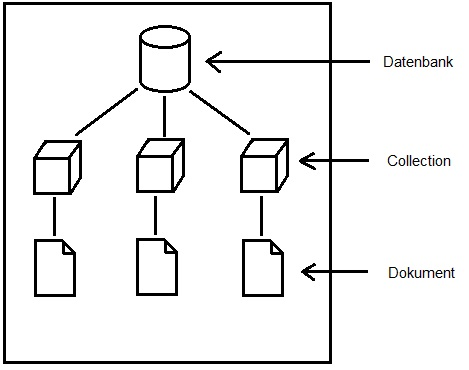
\includegraphics[scale=0.9]{images/Datenmodell_Mongo.jpg}
    \captionof{figure}{Datenbankstruktur von MongoDB}
    \label{fig:ver}
\end{minipage}
\\
Die Collection kann man wie eine Tabelle in einer relationalen Datenbank ansehen und die Dokumente sind die jeweiligen Reihen, also die konkrete Dateneintragungen in die Tabelle.
\subsection{Geschichte}
MongoDB wurde von Dwight Merriman, Eliot Horowitz und seinem Team erstellt. Doch dies nicht auf direktem Wege. 2007 plante das MongoDB Team ein Onlineservice für Web-Anwendungen. Dieser Service sollte die Möglichkeit bieten, eine Web-Anwendung zu entwickeln, zu hosten und zu skalieren. Aufgrund von einem nicht geeigneten Datenbanksystem entschloss sich das Team ein eigenes Datenbanksystem zu erstellen und zu nutzen. Diese hatte noch keinen Namen, da dieses System speziell für den Service des Teams erstellt wurde. Im Jahre 2008 wurde dann das Datenbanksystem fertiggestellt. 2009 entschloss sich das Team, dieses Datenbanksystem, was sie erstellt haben, als Open Source Produkt freizugeben. Dieses System wurde als MongoDB veröffentlicht. März 2010 kam die erste Version von MongoDB heraus, die man in einem größeren Umfang verwenden kann. Über die Jahre wurde MongoDB von dem Team weiterentwickelt und ist zurzeit mit der Version 3.2 veröffentlicht. 
\subsubsection{Philosophie}
Die Philosophie von MongoDB ist im Vergleich zu den meisten anderen etwas unterschiedlich. Denn das Team von MongoDB hat sich dazu entschieden, dass MongoDB nicht die Lösung für jedes Problem sein soll. MongoDB soll eine Lösung für Analytische Probleme und komplexe Datenstrukturen. Zudem liegt der Fokus auf die Nutzung von Dokumenten, nicht auf Zeilen. Das MongoDB Team wollte ein Datenbanksystem was sehr schnell, gut skalierbar und einfach anzuwenden ist.
\subsection{Anwendungsfälle}
MongoDB wird von verschiedenen Unternehmen zu verschiedensten Anwendungen und Aufgaben verwendet.
MTV verwendet MongoDB als Haupt-repository für das MTV-Network.
SourceForge verwendet MongoDB als Back-End Speicher.
Bit.ly verwendet MongoDB, um den Verlauf von Nutzern zu speichern.
New York Times verwendet MongoDB  für eine Foto-Abgabe.
\subsection{Einrichtung}
MongoDB wird für alle Betriebssysteme angeboten und ist derzeit in der Version 3.2 erhältlich. Dadurch lässt sich MongoDB auf Ubuntu 12.04+, Windows Server 2008+ und Mac OS X 10.7+ installieren und verwenden. 
Um MongoDB auf einem Linux Ubuntu Server zu installieren, muss man folgende Schritte befolgen:
\\
\\
1. Importierung von dem public key durch das package management System.
\\
2. Ein Listen-Datei für MongoDB erstellen.
\\
3. Lokale Dateien aktualisieren.
\\
4. Installation von MongoDB Paket.
\\
\\
Um MongoDB auf einem Windows Server zu installieren, muss man wie folgt vorgehen:
\\
\\
1. Bestimmen, welchen Build von MongoDB benötigt wird.
\\
2. MongoDB für Windows runterladen.
\\
3. Installation von MongoDB via Asministrator Kommandozeile.
\\
\\
Um MongoDB auf einem Mac OS System zu installieren, sind folgende Schritte notwendig:
\\
\\
1. Binäre Dateien von der benötigten MongoDB Version runterladen.
\\
2. Heruntergeladene Dateien extrahieren.
\\
3. Extrahierte Dateien in das Zielverzeichnis kopieren.
\\
4. Pfad von MongoDB sicherstellen.
\\
\\
Alle Vorgehensweisen für die Installation von MongoDB verwenden eine Kommandozeile.
%\subsubsection{Indexierung}
\subsubsection{Referenzierung}
Die Referenzierung von MongoDB unterscheidet sich von der Referenzierung von den relationalen Datenbanken. Eine Möglichkeit der Referenzierung in MongoDB wäre die Verschachtlung, also ein Dokument in einem Dokumenten schreiben. Damit kann man die Referenz auf ein anderes Objekt direkt erkennen, was auch für das System einfacher ist, an diese Daten zu gelangen. Das Problem hierbei kann aber eine zu starke Verschachtelungsstruktur sein, was auf Kosten der Übersichtlichkeit geht, zusätzlich wird für ein Dokument mehr Platz gebraucht, da in einem Dokument ein weiteres existiert. Die zweite Möglichkeit für eine Referenzierung, wäre der Verweis auf das jeweilige Dokument. Das verbessert die Übersicht und man kann erkennen, voraus die Daten herkommen. Ein Problem was MongoDB mit sich bringt, ist, dass es keine Direktreferenzierung gibt. In der Relationalen Datenbank kann man mit dem JOIN Befehl die Referenz zu einem anderen Datensatz in Bezug auf einen anderen Datensatz direkt ansprechen und anzeigen lassen. Dies kann MongoDB nicht. Um dies zu ermöglichen, muss man das in einer eigenen Applikation programmieren. 
\subsubsection{Replikation}
Eine Replikation bei MongoDB ist die Kopie von Daten auf weiteren Servern. Dies nennt man replica set. Ein replica set umfasst Server mit derselben Funktionalität und Dient zur Stabilisierung der Aufgabe des jeweiligen replica sets. Die MongoDB Website empfiehlt das Verwenden von drei Servern pro replica set, um somit die Ausfallrate gering zu halten. Die Daten in einem replica set sind auf allen Servern identisch. MongoDB verwendet das Master-Slave System für die Replikation von Daten innerhalb des replica sets. In dem replica set gibt es genau einen Primary und beliebig viele Secondary Server und ggf. einen Arbiter. Datenänderungen wie z.B. Schreiboperationen werden auf dem Primary Server in dem replica set durchgeführt. Nachdem die Operation erfolgreich beendet wurde, übernehmen die Secondary Server die Änderung von dem Primary Server. Sollte der Primary Server ausfallen, so wählen die Secondary Server einen neuen Primary Server aus. Man ist in der Lage, in dem replica set einen Arbiter hinzuzufügen. Ein Arbiter besitzt nicht die Daten, die in dem replica set verteilt werden. Der Arbiter dient lediglich dazu, nur bei einer Abstimmung eine Stimme abzugeben, damit eventuelle Probleme bei einer Abstimmung vermieden werden können. Ein Arbiter selber kann nicht zu einem Primary oder Secondary Server ernannt werden.
\\
\\
\begin{minipage}{\textwidth}
    \centering
    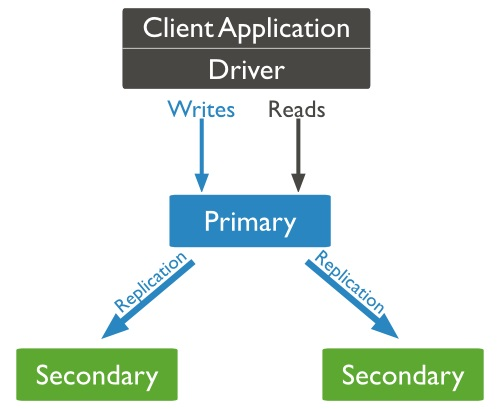
\includegraphics[scale=0.9]{images/replica-set-read-write-operations-primary.jpg}
    \captionof{figure}{Replikationsaufbau von MongoDB}
    \label{fig:ver}
\end{minipage}
\subsubsection{Cluster Sharding}
Ein sharded Cluster bei MongoDB ist eine Methode, um Daten auf unterschiedlichen Servern zu speichern und dann diese schnell aufzurufen. Ein sharded cluster besteht aus drei Komponenten: Den Config Server, den Query Server und Shards. Um ein sharded cluster einzurichten, braucht man mindestens einen Config Server, einen Query Server und 2 Shards. Dies sieht dann wie folgt aus:
\\
\\
\begin{minipage}{\textwidth}
    \centering
    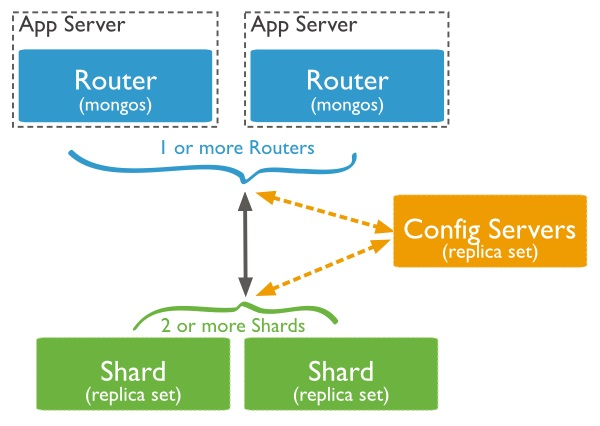
\includegraphics[scale=1.0]{images/sharded-cluster-production-architecture.jpg}
    \captionof{figure}{Aufbau vom Cluster Sharding in MongoDB}
    \label{fig:ver}
\end{minipage}
\\
\\
Config Server: Der Config Server in einem sharded Cluster beinhaltet die Metadaten für dieses. Diese Metadaten beinhalten die Informationen zu der Organisation und die Zustände der jeweiligen Komponenten in dem sharded Cluster.  Ein Config Server ist in einem replica set. Ein replica set verbessert die Konsistenz über die verschiedenen Config Server. Zusätzlich kann man danke dem replica set mehr als 3 Config Server nutzen.
Query Server (Router): Mit dem Query Server ist man in der Lage, Daten auf den verschiedenen Shards zu schreiben und zu Lesen. Dies vollbringt er mit den Metadaten, die der Query Server von dem Config Server bekommt. Der Query Server ist die einzige Schnittstelle in dem sharded Cluster, womit man auf die Daten durch Anwendungen zugreifen kann. 
\\
\\
\begin{minipage}{\textwidth}
    \centering
    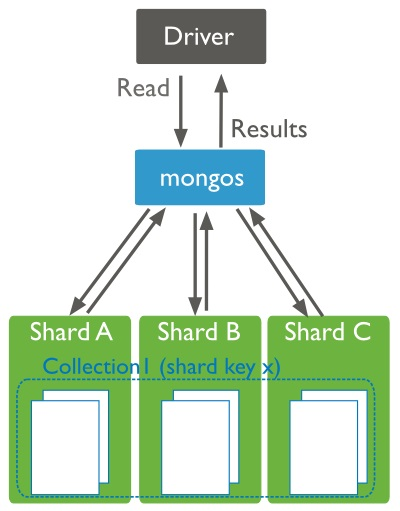
\includegraphics[scale=0.9]{images/sharded-cluster-scatter-gather-query.jpg}
    \captionof{figure}{Datenverteilung von dem Query Server}
    \label{fig:ver}
\end{minipage}
\\
\\
Shard: Bei einer Shard handelt es sich um einen Teil der Gesamtdatenbank. Die Daten, die in die Datenbank eingetragen werden, werden nach den Metadaten des Configservers analysiert und dann durch den Query Server auf das jeweilige Shard gespeichert. Zum Beispiel: Eine 3 Shard Datenbank beinhaltet Daten von Personen in einem Unternehmen. Auf Shard 1 werden alle Mitarbeiter gespeichert, die im Nachnamen mit dem Buchstaben A bis H anfangen. Shard 2 hat den Nachnamen von I bis Q und Shard 3 R bis Z. Dadurch, dass die Daten aufgeteilt und auf unterschiedlichen Shards gespeichert werden, ist man in der Lage schneller an die gewünschten Informationen zu kommen. Shards können sich in einem replica set befinden. Dieses dient für Redundanz  und hohe Verfügbarkeit der Daten.
\subsection{Verwendung}
Um mit MongoDB Daten einzufügen oder auszulesen, sind verschiedene CRUD-Operationen notwendig, wie bei einer relationellen Datenbank. Diese Operationen ähneln wie JavaScript Anweisungen und sind daher leicht anzuwenden. Die wichtigsten Befehle zur Verwendung von MongoDB sind in Tabelle 2.1 zu entnehmen.
\\
\\
\begin{table}[h]
\centering
\begin{tabular}{p{7cm}|p{7cm}|c|c|}
\hline 
Befehl & Funktion \\ 
\hline 
Use <Datenbankname> & Setzt die Datenbank zu den benutzten Namen \\ 
\hline 
db.createCollection(„Name“,{capped : true, size : <byte>, max : <anzahl> }) & Legt eine Collection mit dem angegebenen Namen \\ 
\hline 
db.<name>.insert({Name: „Thomas“, Alter: 25, …})  & Legt ein Dokument in der Collection <name> ab \\ 
\hline 
db.<name>.save({Name: „Thomas“, Alter: 22}) & Einfache Veränderung eines Dokumentes mit dem Namen “Thomas” \\ 
\hline 
db.<name>.update({Name: „Thomas“}, {Name: „Franz“ , Alter: 24}) & Veränderung eines Dokumentes mit dem Namen „Thomas“ \\ 
\hline 
db.<name>.find() & Zeigt alle Dokumente in der Collection <name> \\ 
\hline 
db.<name>.count({Name: „Franz“}) & Zählt alle Dokumente, die den Namen “Franz” beinhalten \\ 
\hline 
db.<name>.remove({Name: “Franz”}) & Löscht alle Dokumente mit dem Namen “Franz” \\ 
\hline 
db.<name>.drop() & Die Collection löschen \\ 
\hline 
\end{tabular}
\caption{Befehlsliste für MongoDB}
\end{table} 
\\
Beim Arbeiten von MongoDB sollte stets geachtet werden, dass man auf der richtigen Datenbank arbeitet und dass die Dokumente in die richtige Collections eingetragen werden. Zudem sollte man auf Groß-  und Kleinschreibung achten, da MongoDB Case-Sensitive ist. 
\subsection{Grenzen}
MongoDB besitzt in mehrere Bereiche Limitationen, die die Performance und das Nutzen von MongoDB einschränken. 
\begin{itemize}
\item 32bit Version von MongoDB kann nur eine Datenbank einrichten, die maximal 2 GB groß sein kann. Dieses Problem kann behoben werden, indem man die 64bit Version von MongoDB verwendet. Zudem wird die 32bit Version von MongoDB nicht mehr seit der 3.0 Version unterstützt.
\item BSON Dokumente können maximal 16MB groß sein, was aber in Vergleich zu anderen Datenbanksystemen sehr groß ist.
\item Indexe in MongoDB können nicht größer als 1024 Byte sein. Zudem kann eine Collection maximal 64 Indexe besitzen. Auch der Name des Indexes ist auf 128 Byte begrenzt. Diese Limitationen sollten bei einer gut aufgebauten Datenbank nicht erreicht werden.
\item Sobald eine Collection mit einer Grenze eingestellt wurde, kann diese nicht erweitert werden. Das maximum was man bei der Grenzeinstellung vornehmen kann ist 232 Dokumente. Man ist aber auch in der Lage, diese Grenze auszustellen. Sollte die Grenze erreicht werden, kann man nur mit einer neuen Collection mit einer größeren oder keiner Grenze das Problem beheben.
\item Das Sharding sollte wenn möglich so früh wie möglich eingeführt werden, da sonst die Performance von MongoDB stark beeinträchtigt wird, da die Server die Daten auf den unterschiedlichen Shards verteilen muss. Zudem sollte auch geachtet werden, das die Datenbank nicht über 256 GB groß ist, da MongoDB bei einer Größe von 256 GB das Sharding nicht mehr erlaubt.
\item Die Daten die bei MongoDB versendet werden sind nicht verschlüsselt.
Bei Lese und Schreibvorgänge bei der MongoDB muss man auf Groß- und Kleinschreibung achten, da MongoDB Case-Sensitive ist.
\item MongoDB besitzt keine JOIN-Operation. Man muss diese durch verschachtelte Dokumente oder auf einen verweis auf das jeweilige Dokument machen.
\end{itemize}
\chapter{Ausgewählte Anwendungsszenarien}
\section{Web 2.0 - Abschlussarbeiten-DB}
Im Rahmen dieses Einführungsprojektes in gängige NoSQL ist ein relationales Schema gegeben, dass auf das jeweilige NoSQL äquivalent portiert werden soll. Zusätzlich sind Datensätze gegeben, die in den jeweiligen Datenbanken eingefügt werden sollen. 

\subsection{Das semantische Schema}
In der Abbildung \ref{fig:schema1} ist das Schema der Datenbank zu sehen, die in den gängigen NoSQL Techniken umgesetzt werden soll. Eine Abschlussarbeit wird von einem Studenten oder einem Auszubildenden geschrieben. In Auftrag gegeben wird die Arbeit von einer Organisation, die eine Universität oder ein Unternehmen sein kann. Die Arbeit wird eventuell von Erstprüfern und Zweitprüfern begutachtet. Der mit der Arbeit verbunden Abschluss hat einen Titel. Das Thema der Arbeit kann in einer Kategorie liegen, in der auch der Prüfer oder das Unternehmen liegen.\\

Insgesamt sind 27 Klassen gegeben, auf denen 36 Attribute verteilt sind. Im Zentrum des Schemas steht der Abschluss ("Degree"). Hier kommen alle wichtigen Informationen zusammen. \\

\begin{figure}[H]
	\centering
	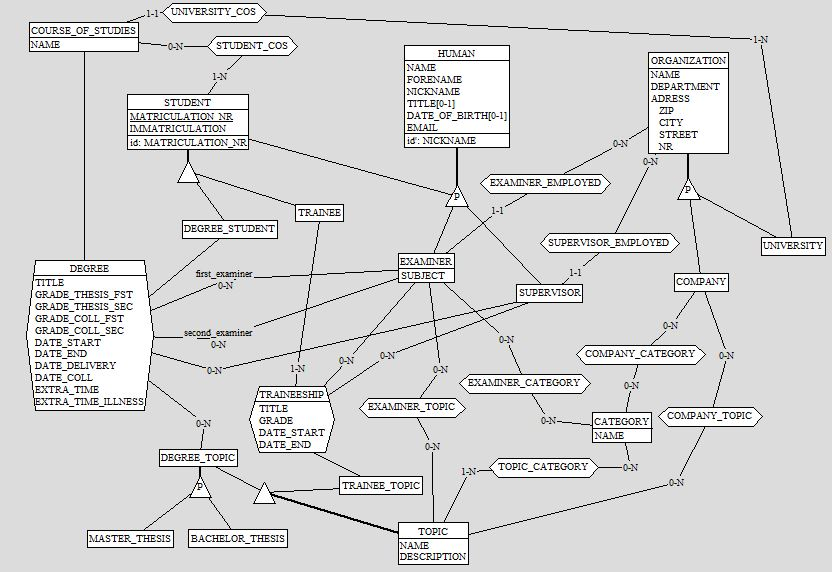
\includegraphics[scale=0.6]{images/abschlussarbeitendbschema.jpg} 
	\caption{AbschlussarbeitenDB Schema}\label{fig:schema1}
\end{figure}

\subsection{Die Datenbestände}

\begin{figure}[H]
	\centering
	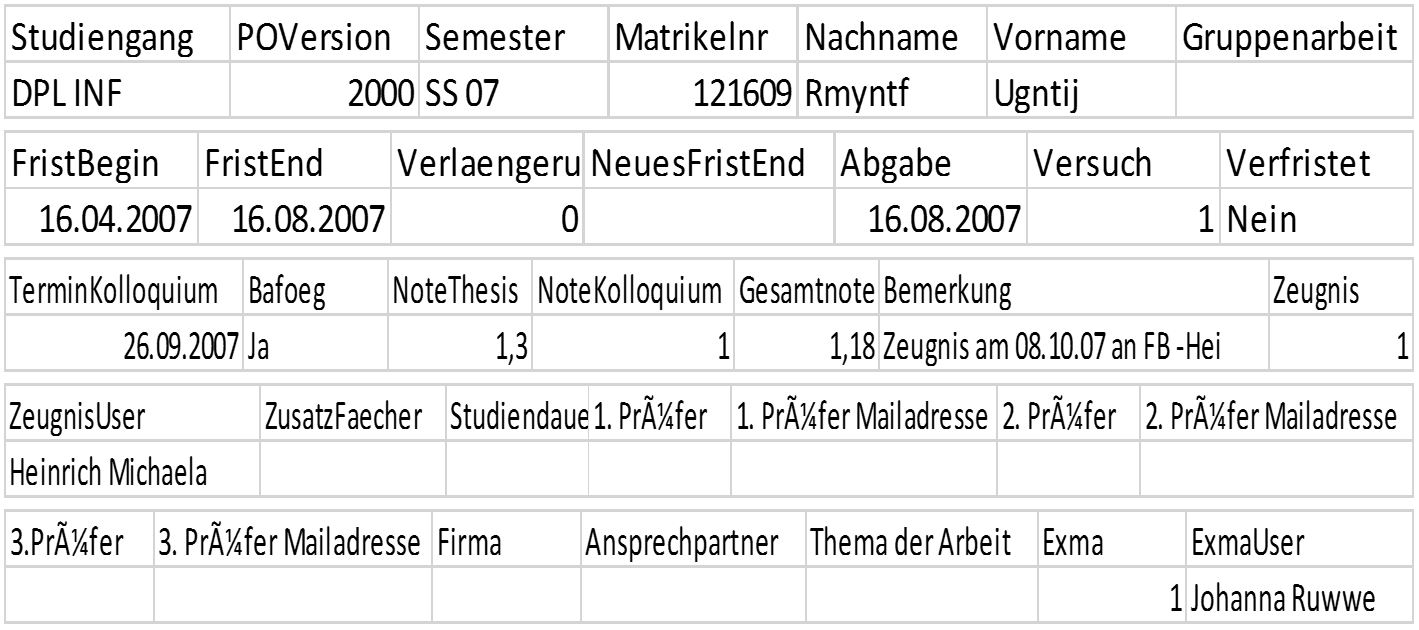
\includegraphics[scale=0.3]{images/beispieldatensatzcsv.jpg} 
	\caption{Beispiel-Datensatz}\label{fig:schema2}
\end{figure}

\section{MongoDB}


%\chapter{Erstes Kapitel}
Das ist zunächst ein normaler Text ... Lorem ipsum dolor sit amet, consetetur sadipscing elitr, sed diam nonumy eirmod tempor invidunt ut labore et dolore magna aliquyam erat, sed diam voluptua. At vero eos et accusam et justo duo dolores et ea rebum. Stet clita kasd gubergren, no sea takimata sanctus est Lorem ipsum dolor sit amet. Lorem ipsum dolor sit amet, consetetur sadipscing elitr, sed diam nonumy eirmod tempor invidunt ut labore et dolore magna aliquyam erat, sed diam voluptua. At vero eos et accusam et justo duo dolores et ea rebum. Stet clita kasd gubergren, no sea takimata sanctus est Lorem ipsum dolor sit amet. Lorem ipsum dolor sit amet, consetetur sadipscing elitr, sed diam nonumy eirmod tempor invidunt ut labore et dolore magna aliquyam erat, sed diam voluptua. At vero eos et accusam et justo duo dolores et ea rebum. Stet clita kasd gubergren, no sea takimata sanctus est Lorem ipsum dolor sit amet. 

Duis autem vel eum iriure dolor in hendrerit in vulputate velit esse molestie consequat, vel illum dolore eu feugiat nulla facilisis at vero eros et accumsan et iusto odio dignissim qui blandit praesent luptatum zzril delenit augue duis dolore te feugait nulla facilisi. Lorem ipsum dolor sit amet, consectetuer adipiscing elit, sed diam nonummy nibh euismod tincidunt ut laoreet dolore magna aliquam erat volutpat. 

Lorem ipsum dolor sit amet, consetetur sadipscing elitr, sed diam nonumy eirmod tempor invidunt ut labore et dolore magna aliquyam erat, sed diam voluptua. At vero eos et accusam et justo duo dolores et ea rebum. Stet clita kasd gubergren, no sea takimata sanctus est Lorem ipsum dolor sit amet. 
\begin{center}
Der folgende Bereich (Umgebung) \\ 
wird jetzt zentriert (center von begin bis end)
\Large

und zugleich groß (Large)
\tiny

und jetzt zugleich klein (tiny)
\end{center}
Es wird lediglich das folgende Wort
\textsl{kursiv} (textsl, slanted) hervorgehoben. 

Das folgende Word wird \textbf{fett} (textbf, boldface) und jetzt \textsl{\textbf{fett und kursiv}} zugleich dargestellt.

Ein Textbereich kann auch ab jetzt \itshape (z.B. itshape, kursiv) hervorgehoben werden ... solange bis eine andere Hervorhebung wie z.B. das \normalfont Standardformat (normalfont) wieder festgelegt wird. 

Sonderzeichen müssen gekennzeichnet bzw. maskiert werden:

\verb=\=: ganz kompliziert mit \bfseries \verb=\=verb=\verb=\== \normalfont

\verb=~=: ebenfalls kompliziert mit \bfseries \verb=\=verb=\verb=~== \normalfont

Viele Sonderzeichen benötigen jedoch nur ein vorangestelltes \verb=\=:

\%: \bfseries \verb=\=\% \normalfont

\{: \bfseries \verb=\=\{ \normalfont

\_: \bfseries \verb=\=\- \normalfont

Die Befehle für deutsche Anführungszeichen sind Teil des Pakets german, bzw. ngerman. Das untere Anführungszeichen erhält man durch "'`, das obere durch "''.

Die deutschen Umlaute werden durch das Einbinden entsprechender Zusatzmodule (Pachages) für die deutschen Schriftzeichen ermöglicht und können "`einfach so"' benutzt werden: äöüÄÖÜß.

Einen einfachen Umbruch (jetzt)\\ in einem Absatz erreicht man mit \verb=\=\verb=\=. 

Jetzt kommt eine Fußnote.\footnote{http://www.h-brs.de}

\section{Listings}
Jetzt kommen einige Listings, die exakt dort im Text erscheinen, wo sie definiert werden. Das Problem hierbei ist, dass die Listings Opfer des Seitenumbruchs werden können. Abhilfe schafft hier die Option "`float, floatplacement=H"', wodurch das Listing an den Anfang der nächsten Seite gesetzt wird. Bei Tabellen und Abbildungen wird eine andere dynamische Positionierung genutzt (siehe Abbildung \ref{figure01} und Tabelle \ref{table01} im zweiten Kapitel ).

\lstsethaskell
\begin{lstlisting}[float, floatplacement=H, label=listinghaskell, captionpos=b, caption=Beispiel Haskell]
module Main where

-- this is a comment
f :: Show a => a -> Int -> String
f x i = show x ++ show i

main :: IO ()
main = do
  putStrLn "Hello World"
  putStrLn $ f 1.2 3
  print $ sum [1..10]
\end{lstlisting}

Lorem ipsum dolor sit amet, consetetur sadipscing elitr, sed diam nonumy eirmod tempor invidunt ut labore et dolore magna aliquyam erat, sed diam voluptua. At vero eos et accusam et justo duo dolores et ea rebum. Stet clita kasd gubergren, no sea takimata sanctus est Lorem ipsum dolor sit amet.
 
\lstsetjava
\begin{lstlisting}[float, floatplacement=H, label=listingjava,caption=Beispiel Java]
// Comment
class Main {
  public static void main(String[] args) {
    System.out.println("Hello World");
  }
}
\end{lstlisting}

Lorem ipsum dolor sit amet, consetetur sadipscing elitr, sed diam nonumy eirmod tempor invidunt ut labore et dolore magna aliquyam erat, sed diam voluptua. 

\lstsetscala
\begin{lstlisting}[label=listingscala,caption=Beispiel Scala]
// Comment
class Main extends App {
  println("Hello World")
}
\end{lstlisting}

\section{Formeln}

Komplette Referenz zu AMSMath siehe \\
\url{ftp://ftp.ams.org/ams/doc/amsmath/short-math-guide.pdf}

\begin{align}
 \int_{a}^{b} x\,dx
 & = \left.\frac{1}{2} x^2\right\vert_{a}^{b}\\
 & = \frac{1}{2} b^2 - \frac{1}{2} a^2 \\
 \intertext{mit $a=1$ und $b=3$ folgt:}
 \notag
 & = \frac{1}{2} \left(3^2 - 1^2\right)\\
 & = 5
\end{align}

\section{Dritter Abschnitt}
Lorem ipsum dolor sit amet, consetetur sadipscing elitr, sed diam nonumy eirmod tempor invidunt ut labore et dolore magna aliquyam erat, sed diam voluptua. At vero eos et accusam et justo duo dolores et ea rebum. Stet clita kasd gubergren, no sea takimata sanctus est Lorem ipsum dolor sit amet. Lorem ipsum dolor sit amet, consetetur sadipscing elitr, sed diam nonumy eirmod tempor invidunt ut labore et dolore magna aliquyam erat, sed diam voluptua. At vero eos et accusam et justo duo dolores et ea rebum. Stet clita kasd gubergren, no sea takimata sanctus est Lorem ipsum dolor sit amet. Lorem ipsum dolor sit amet, consetetur sadipscing elitr, sed diam nonumy eirmod tempor invidunt ut labore et dolore magna aliquyam erat, sed diam voluptua. At vero eos et accusam et justo duo dolores et ea rebum. Stet clita kasd gubergren, no sea takimata sanctus est Lorem ipsum dolor sit amet. 

Jetzt kommt eine Referenz \cite[Seite 300]{kudrass01}

\section{Vierter Abschnitt}
Lorem ipsum dolor sit amet, consetetur sadipscing elitr, sed diam nonumy eirmod tempor invidunt ut labore et dolore magna aliquyam erat, sed diam voluptua. At vero eos et accusam et justo duo dolores et ea rebum. Stet clita kasd gubergren, no sea takimata sanctus est Lorem ipsum dolor sit amet. Lorem ipsum dolor sit amet, consetetur sadipscing elitr, sed diam nonumy eirmod tempor invidunt ut labore et dolore magna aliquyam erat, sed diam voluptua. At vero eos et accusam et justo duo dolores et ea rebum. Stet clita kasd gubergren, no sea takimata sanctus est Lorem ipsum dolor sit amet. Lorem ipsum dolor sit amet, consetetur sadipscing elitr, sed diam nonumy eirmod tempor invidunt ut labore et dolore magna aliquyam erat, sed diam voluptua. At vero eos et accusam et justo duo dolores et ea rebum. Stet clita kasd gubergren, no sea takimata sanctus est Lorem ipsum dolor sit amet. 

\section{Noch ein Abschnitt}
Lorem ipsum dolor sit amet, consetetur sadipscing elitr, sed diam nonumy eirmod tempor invidunt ut labore et dolore magna aliquyam erat, sed diam voluptua. At vero eos et accusam et justo duo dolores et ea rebum. Stet clita kasd gubergren, no sea takimata sanctus est Lorem ipsum dolor sit amet. Lorem ipsum dolor sit amet, consetetur sadipscing elitr, sed diam nonumy eirmod tempor invidunt ut labore et dolore magna aliquyam erat, sed diam voluptua. At vero eos et accusam et justo duo dolores et ea rebum. Stet clita kasd gubergren, no sea takimata sanctus est Lorem ipsum dolor sit amet. Lorem ipsum dolor sit amet, consetetur sadipscing elitr, sed diam nonumy eirmod tempor invidunt ut labore et dolore magna aliquyam erat, sed diam voluptua. At vero eos et accusam et justo duo dolores et ea rebum. Stet clita kasd gubergren, no sea takimata sanctus est Lorem ipsum dolor sit amet. 

Und noch eine Fußnote, jetzt mit Referenz: \footnote{Vgl. \cite{redmont01}}

\section{Ein Abschnitt zweiten Grades}
Lorem ipsum dolor sit amet, consetetur sadipscing elitr, sed diam nonumy eirmod tempor invidunt ut labore et dolore magna aliquyam erat, sed diam voluptua. At vero eos et accusam et justo duo dolores et ea rebum. Stet clita kasd gubergren, no sea takimata sanctus est Lorem ipsum dolor sit amet. Lorem ipsum dolor sit amet, consetetur sadipscing elitr, sed diam nonumy eirmod tempor invidunt ut labore et dolore magna aliquyam erat, sed diam voluptua. At vero eos et accusam et justo duo dolores et ea rebum. Stet clita kasd gubergren, no sea takimata sanctus est Lorem ipsum dolor sit amet. Lorem ipsum dolor sit amet, consetetur sadipscing elitr, sed diam nonumy eirmod tempor invidunt ut labore et dolore magna aliquyam erat, sed diam voluptua. At vero eos et accusam et justo duo dolores et ea rebum. Stet clita kasd gubergren, no sea takimata sanctus est Lorem ipsum dolor sit amet. 
\subsection{Ein Abschnitt dritten Grades}
Lorem ipsum dolor sit amet, consetetur sadipscing elitr, sed diam nonumy eirmod tempor invidunt ut labore et dolore magna aliquyam erat, sed diam voluptua. At vero eos et accusam et justo duo dolores et ea rebum. Stet clita kasd gubergren, no sea takimata sanctus est Lorem ipsum dolor sit amet. Lorem ipsum dolor sit amet, consetetur sadipscing elitr, sed diam nonumy eirmod tempor invidunt ut labore et dolore magna aliquyam erat, sed diam voluptua. At vero eos et accusam et justo duo dolores et ea rebum. Stet clita kasd gubergren, no sea takimata sanctus est Lorem ipsum dolor sit amet. Lorem ipsum dolor sit amet, consetetur sadipscing elitr, sed diam nonumy eirmod tempor invidunt ut labore et dolore magna aliquyam erat, sed diam voluptua. At vero eos et accusam et justo duo dolores et ea rebum. Stet clita kasd gubergren, no sea takimata sanctus est Lorem ipsum dolor sit amet. 
\subsubsection{Ein Abschnitt vierten Grades}
Lorem ipsum dolor sit amet, consetetur sadipscing elitr, sed diam nonumy eirmod tempor invidunt ut labore et dolore magna aliquyam erat, sed diam voluptua. At vero eos et accusam et justo duo dolores et ea rebum. Stet clita kasd gubergren, no sea takimata sanctus est Lorem ipsum dolor sit amet. Lorem ipsum dolor sit amet, consetetur sadipscing elitr, sed diam nonumy eirmod tempor invidunt ut labore et dolore magna aliquyam erat, sed diam voluptua. At vero eos et accusam et justo duo dolores et ea rebum. Stet clita kasd gubergren, no sea takimata sanctus est Lorem ipsum dolor sit amet. Lorem ipsum dolor sit amet, consetetur sadipscing elitr, sed diam nonumy eirmod tempor invidunt ut labore et dolore magna aliquyam erat, sed diam voluptua. At vero eos et accusam et justo duo dolores et ea rebum. Stet clita kasd gubergren, no sea takimata sanctus est Lorem ipsum dolor sit amet. 
\subsubsection{Noch ein Abschnitt vierten Grades}
Es sollten immer mindestens zwei Unterabschnitte auf einer Ebene vorhanden sein. Lorem ipsum dolor sit amet, consetetur sadipscing elitr, sed diam nonumy eirmod tempor invidunt ut labore et dolore magna aliquyam erat, sed diam voluptua. At vero eos et accusam et justo duo dolores et ea rebum. Stet clita kasd gubergren, no sea takimata sanctus est Lorem ipsum dolor sit amet. Lorem ipsum dolor sit amet, consetetur sadipscing elitr, sed diam nonumy eirmod tempor invidunt ut labore et dolore magna aliquyam erat, sed diam voluptua. At vero eos et accusam et justo duo dolores et ea rebum. Stet clita kasd gubergren, no sea takimata sanctus est Lorem ipsum dolor sit amet. Lorem ipsum dolor sit amet, consetetur sadipscing elitr, sed diam nonumy eirmod tempor invidunt ut labore et dolore magna aliquyam erat, sed diam voluptua. At vero eos et accusam et justo duo dolores et ea rebum. Stet clita kasd gubergren, no sea takimata sanctus est Lorem ipsum dolor sit amet. 
\paragraph{Ein Abschnitt ohne expliziten Grad}
Lorem ipsum dolor sit amet, consetetur sadipscing elitr, sed diam nonumy eirmod tempor invidunt ut labore et dolore magna aliquyam erat, sed diam voluptua. At vero eos et accusam et justo duo dolores et ea rebum. Stet clita kasd gubergren, no sea takimata sanctus est Lorem ipsum dolor sit amet. Lorem ipsum dolor sit amet, consetetur sadipscing elitr, sed diam nonumy eirmod tempor invidunt ut labore et dolore magna aliquyam erat, sed diam voluptua. At vero eos et accusam et justo duo dolores et ea rebum. Stet clita kasd gubergren, no sea takimata sanctus est Lorem ipsum dolor sit amet. Lorem ipsum dolor sit amet, consetetur sadipscing elitr, sed diam nonumy eirmod tempor invidunt ut labore et dolore magna aliquyam erat, sed diam voluptua. At vero eos et accusam et justo duo dolores et ea rebum. Stet clita kasd gubergren, no sea takimata sanctus est Lorem ipsum dolor sit amet. 
\subsection{Ein zweiter Abschnitt dritten Grades}
Es sollten immer mindestens zwei Unterabschnitte auf einer Ebene vorhanden sein. Lorem ipsum dolor sit amet, consetetur sadipscing elitr, sed diam nonumy eirmod tempor invidunt ut labore et dolore magna aliquyam erat, sed diam voluptua. At vero eos et accusam et justo duo dolores et ea rebum. Stet clita kasd gubergren, no sea takimata sanctus est Lorem ipsum dolor sit amet. Lorem ipsum dolor sit amet, consetetur sadipscing elitr, sed diam nonumy eirmod tempor invidunt ut labore et dolore magna aliquyam erat, sed diam voluptua. At vero eos et accusam et justo duo dolores et ea rebum. Stet clita kasd gubergren, no sea takimata sanctus est Lorem ipsum dolor sit amet. Lorem ipsum dolor sit amet, consetetur sadipscing elitr, sed diam nonumy eirmod tempor invidunt ut labore et dolore magna aliquyam erat, sed diam voluptua. At vero eos et accusam et justo duo dolores et ea rebum. Stet clita kasd gubergren, no sea takimata sanctus est Lorem ipsum dolor sit amet. 




%\chapter{Zweites Kapitel}
Lorem ipsum dolor sit amet, consetetur sadipscing elitr, sed diam nonumy eirmod tempor invidunt ut labore et dolore magna aliquyam erat, sed diam voluptua. At vero eos et accusam et justo duo dolores et ea rebum. Stet clita kasd gubergren, no sea takimata sanctus est Lorem ipsum dolor sit amet. Lorem ipsum dolor sit amet, consetetur sadipscing elitr, sed diam nonumy eirmod tempor invidunt ut labore et dolore magna aliquyam erat, sed diam voluptua. At vero eos et accusam et justo duo dolores et ea rebum. Stet clita kasd gubergren, no sea takimata sanctus est Lorem ipsum dolor sit amet. Lorem ipsum dolor sit amet, consetetur sadipscing elitr, sed diam nonumy eirmod tempor invidunt ut labore et dolore magna aliquyam erat, sed diam voluptua. At vero eos et accusam et justo duo dolores et ea rebum. Stet clita kasd gubergren, no sea takimata sanctus est Lorem ipsum dolor sit amet.

Jetzt kommt eine Abbildung (siehe Abbildung \ref{figure01}). Damit sie ebenfalls nicht Opfer eines Seitenumbruchs wird, erscheint sie unten (b-ottom) auf der aktuellen Seite oben.

\begin{figure}[b]

\begin{center}
  	
\includegraphics[scale=1]{images/Logo_H-BRS.jpg}
\end{center}

\caption{Eine Abbildung, die unten erscheint}
\label{figure01}
\end{figure} 

Jetzt kommen Aufzählungen mit Spiegelstrich (itemize):
\begin{itemize}
\item
Lorem ipsum dolor sit amet, consetetur sadipscing elitr, sed diam nonumy eirmod tempor invidunt ut labore
   \begin{itemize}
   \item
Lorem ipsum dolor sit amet, consetetur sadipscing elitr, sed diam nonumy eirmod tempor invidunt ut labore
      \begin{itemize}
      \item
Lorem ipsum dolor sit amet, consetetur sadipscing elitr, sed diam nonumy eirmod tempor invidunt ut labore
      \item
et dolore magna aliquyam erat, sed diam voluptua. At vero eos et accusam et justo duo dolores et ea rebum. Stet clita kasd gubergren
      \item
no sea takimata sanctus est Lorem ipsum dolor sit amet
      \end{itemize}
\item
et dolore magna aliquyam erat, sed diam voluptua. At vero eos et accusam et justo duo dolores et ea rebum. Stet clita kasd gubergren
   \item
no sea takimata sanctus est Lorem ipsum dolor sit amet
   \end{itemize}
\item
et dolore magna aliquyam erat, sed diam voluptua. At vero eos et accusam et justo duo dolores et ea rebum. Stet clita kasd gubergren
\item
no sea takimata sanctus est Lorem ipsum dolor sit amet
\end{itemize}

Jetzt kommt eine einfache Tabelle  (siehe Tabelle \ref{table01}) mit drei Spalten. Damit sie nicht Opfer eines Seitenumbruchs wird, erscheint sie oben (t-op) auf der aktuellen oder nachfolgenden Seite.

\begin{table}[t]

\begin{tabular}{|c|l|r|}
\hline
Spalte 1 (zentriert)& Spalte 2 (links)& Spalte 3 (rechts)\\
\hline
\hline
1 & et dolore magna aliquyam & 1001 \\
\hline
2 & sanctus est Lorem ipsum dolor & 1002 \\
\hline
3 & justo duo dolores et ea rebum & 1003 \\
\hline
4 & no sea takimata sanctus est Lorem & 1004 \\
\hline
5 & sed diam voluptua & 1005 \\
\hline
6 & clita kasd gubergren & 1006 \\
\hline
\end{tabular}

\caption{Eine Tabelle, die oben erscheint}
\label{table01}
\end{table}

Jetzt kommen Aufzählungen mit Nummerierungen mit (enumerate):
\begin{enumerate}
\item
Lorem ipsum dolor sit amet, consetetur sadipscing elitr, sed diam nonumy eirmod tempor invidunt ut labore
   \begin{enumerate}
   \item
Lorem ipsum dolor sit amet, consetetur sadipscing elitr, sed diam nonumy eirmod tempor invidunt ut labore
      \begin{enumerate}
      \item
Lorem ipsum dolor sit amet, consetetur sadipscing elitr, sed diam nonumy eirmod tempor invidunt ut labore
      \item
no sea takimata sanctus est Lorem ipsum dolor sit amet
      \end{enumerate}
\item
et dolore magna aliquyam erat, sed diam voluptua. At vero eos et accusam et justo duo dolores et ea rebum. Stet clita kasd gubergren
   \item
no sea takimata sanctus est Lorem ipsum dolor sit amet
   \end{enumerate}
\item
et dolore magna aliquyam erat, sed diam voluptua. At vero eos et accusam et justo duo dolores et ea rebum. Stet clita kasd gubergren
\item
no sea takimata sanctus est Lorem ipsum dolor sit amet
\end{enumerate}


\newpage

% loads the fancy pagestyle for register part
% set the pagestyle to fancy
\pagestyle{fancy}

\fancyhf{}% clear all fields
  % define the header
  \fancyhead[L]{\leftmark}% left header
  \fancyhead[R]{\HEADER}% right header
  \renewcommand{\headrulewidth}{0.4pt}% top line

  % define the footer
  \fancyfoot[L]{\AUTHOR}% left footer
  \fancyfoot[R]{\pagemark}% right footer
  \renewcommand{\footrulewidth}{0.6pt}% bottom line

  % redefine the chaptermark to have '1. Chaptername' and not 'CHAPTER 1.
  % CHAPTERNAME'
  \renewcommand{\chaptermark}[1]{\markboth{\thechapter.\ #1}{}}

% override the plain style
\fancypagestyle{plain}{%
\fancyhf{}% clear all fields
  % define the header
  \renewcommand{\headrulewidth}{0.0pt}% top line

  % define the footer
  \fancyfoot[L]{\AUTHOR}% left footer
  \fancyfoot[R]{\pagemark}% right footer
  \renewcommand{\footrulewidth}{0.6pt}% bottom line
}


% #####
% # load the appendix from the files
% #####
% \appendix
\chapter{Anhang}
Appendix
\section{Erster Teil}
\section{Zweiter Teil}
\chapter{Anhang}
Appendix


% #####
% # list of table, list of figures, and list of listings in ToC
% #####
%\newpage
%\addcontentsline{toc}{chapter}{Abbildungsverzeichnis}
%\listoffigures
%\newpage
%\addcontentsline{toc}{chapter}{Tabellenverzeichnis}
%\listoftables
%\newpage
%\addcontentsline{toc}{chapter}{Listings}
%\lstlistoflistings

% #####
% # List of Abbreviations
% #####
%\phantomsection 
%\addcontentsline{toc}{chapter}{Abkürzungsverzeichnis}
%\renewcommand\refname{Abkürzungsverzeichnis} 
%\chapter*{Abkürzungsverzeichnis}
%\begin{acronym}[RDBMS] % längste Abkürzung steht in eckigen Klammern
    \setlength{\itemsep}{-\parsep} % geringerer Zeilenabstand
    \acro{API}{Application Programming Interface}
    \acro{BASE}{Basically Available, Soft State, Eventual Consistency}
    \acro{BG}{Barahmand Ghandeharizadeh}
    \acro{CAP}{Consistency Availibiltiy Partition Tolerance}
    \acro{CLI}{Command-Line Interface}
    \acro{CPU}{Central Processing Unit}
    \acro{CRUD}{Create, Read, Update, Delete}
    \acro{DBA}{Datenbankadministrator}
    \acro{DBS}{Datenbanksystem}
    \acrodefplural{DBS}[DBS]{Datenbanksysteme}
    \acrodefplural{HDD}[HDDs]{Hard Disk Drive}
    \acrodefplural{SSD}[SSDs]{Solid State Drive}
    \acro{DNS}{Domain Name System}
    \acro{DTD}{Document Type Definition}
    \acro{GUI}{Graphical User Interface}
    \acro{HDD}{Hard Disk Drive}
    \acro{IP}{Internet Protocol}
    \acro{JDBC}{Java Database Connectivity}
    \acro{JSON}{JavaScript Object Notation}
    \acro{NoSQL}{Not only SQL}
    \acro{OLTP}{Online Transaction Processing}
    \acro{RDBMS}{Relational Database Management System}
    \acro{RFC}{Request For Comments}
    \acro{SLA}{Service Level Agreement}
    \acro{SPEC}{Standard Performance Evaluation Corporation}
    \acro{SQL}{Structured Query Language}
    \acro{SSD}{Solid State Drive}
    \acro{TPC}{Transaction Processing Performance Council}
    \acro{UML}{Unified Markup Language}
    \acro{XML}{Extensible Markup Language}
    \acro{YCSB}{Yahoo! Cloud Serving Benchmark}
\end{acronym}

%\newpage

% #####
% # load the bibliography
% #####
\bibliography{bibliography}

% #####
% # load the sworn declaration
% #####
%\chapter*{Eidesstattliche Erklärung}\markboth{Eidesstattliche Erklärung}{}
  \addcontentsline{toc}{chapter}{Eidesstattliche Erklärung}
Ich versichere an Eides Statt durch meine eigenhändige Unterschrift, dass
ich die vorliegende Arbeit selbstständig und ohne fremde Hilfe angefertigt
habe. Alle Stellen, die wörtlich oder dem Sinn nach auf Publikationen oder
Vorträgen anderer Autoren beruhen, sind als solche kenntlich gemacht.
Ich versichere außerdem, dass ich keine andere als die angegebene
Literatur verwendet habe. Diese Versicherung bezieht sich auch auf alle in
der Arbeit enthaltenen Zeichnungen, Skizzen, bildlichen Darstellungen und
dergleichen.
\\
\\
Die Arbeit wurde bisher keiner anderen Prüfungsbehörde vorgelegt und
auch noch nicht veröffentlicht.
\vspace{3cm}

\centering
\begin{tabular}{p{10mm}>{\centering\arraybackslash}p{50mm}p{10mm}
>{\centering\arraybackslash}p{50mm}p{10mm}}
&\textit{\large \TOWN,}&&& \\
&\textit{\large den \today}&&\hrulefill& \\
&\small Ort, Datum&&\small \AUTHOR&
\end{tabular}
% end of the document
\end{document}
